\chapter{Projet Kinect pour une application de peinture à main levée}


\section{Présentation}

Ce projet porte sur l'adaptation d'une application existante (peinture à main levée) qui utilise comme dispositif d'interaction un système de motion capture ARTrack d'un coût élevé. L'objectif est de permettre une interaction par Kinect.

Kinect est l'outil développé par l'entreprise \textit{PrimeSense} et popularisé par \textit{Microsoft}  avec la Xbox 360. Il s'agit d'une caméra permettant de contrôler avec son corps, ou par commande vocale des applications, jeux, etc. PrimeSense fournit des codes Samples permettant d'utiliser les outils de détection de mouvements, de squelettes et de communication vocale. La détection du squelette sera utilisé et plus particullièrement la détection des mains pour pouvoir interagir avec WabinPaint et permettre à l'utilisateur de dessiner.

L'ajout du contrôle via Kinect est pertinent puisqu'il s'agit d'un outil grand public et à faible coût, contrairement aux outils déjà implémenté dans WabinPaint. De plus l'outil Kinect simplifie la mise en place du dispositif puisque aucun réglage n'est nécessaire contrairement aux dispositifs infrarouges qui nécessitent une calibration et un placement défini de l'utilisateur.

L'utilisation de Kinect a pour but la rééducation fonctionnelle. L'application sera utilisée pour des patients atteints d'héminégligence accompagnée de faibles troubles moteurs. L'héminégligence signifie qu'ils ne percoivent qu'une partie de leur environnement et sont donc, par exemple, dans l'incapacité de dessiner la totalité d'un objet. WabinPaint utilisant Kinect, permettra à ces patients de dessiner tout en utilisant leurs gestes, ce qui favorise leurs rééducation fonctionelle.

Le signal produit par la Kinect est fortement bruité (il s'apparente à un tremblement). Un traitement du signal sera effectué grâce au \textit{One Euro Filter}.

\section{WabinPaint}

WabinPaint est une application de dessin développée par l'équipe de recherche MINT comme démonstrateur de ses travaux sur les interactions à mains libres.

Cette application permet à un utilisateur d'utiliser plusieurs méthodes de tracking différentes comme par exemple, une souris, des trackers infrarouges, etc. Wabinpaint permet de dessiner dans un canvas en trois dimensions et propose une rotation du dessin pour visualiser la profondeur.

Plusieurs options de dessin sont également disponibles telles que:
\begin{itemize}
	\item couleur du pinceaux
	\item épaisseur du pinceaux
	\item rotation du canvas
	\item effacement du canvas
\end{itemize}

Voici un rendu de l'application: 
\begin{figure}[!ht]
	\center
	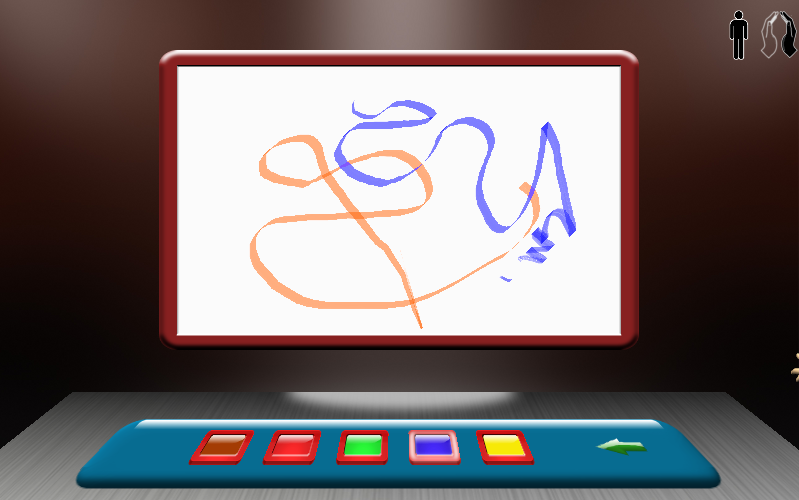
\includegraphics[scale=0.45]{image/wabinpaint.png}
	\caption{Screenshot de WabinPaint}
\end{figure}

\newpage

\section{Objectif}

L'objectif de ce projet est de comprendre comment Kinect fonctionne, d'appliquer des traitements, des lissages sur les cordonnées des mains dans un plan en trois dimensions, pour que l'utilisateur puisse dessiner.

Le projet comportera trois parties distinctes qui sont:
\begin{itemize}
\item Traitement des données Kinect et génération du squelette
\item Récupération de la position des mains et intégration dans WabinPaint
\item Traitement du bruit des positions 
\end{itemize}


\section{Méthodologie de gestion de projet}
Pour concevoir une base logicielle solide et avoir des points de vues différents nous avons (Erwan Douaille \&\ Yoan Miranda) pair-programmé. Le code source du projet est disponible sur la forge de développement de l'équipe MINT.